\documentclass[twoside]{article}
\usepackage{amsmath,amssymb,amsthm,graphicx}
\usepackage{epsfig}
\usepackage[authoryear]{natbib}

\usepackage{geometry}
\usepackage{setspace}

\geometry{twoside,
          letterpaper, % i.e, paperwidth=210mm and paperheight=297mm,
          top=25mm,
          bottom=45mm,
          left=25mm,
          right=25mm,
}

\setlength{\parindent}{0pt}
\setlength{\parskip}{0.5cm}
% Local Macros Put your favorite macros here that don't appear in
% stat-macros.tex.  We can eventually incorporate them into
% stat-macros.tex if they're of general use.

\begin{document}

\textbf{Reflection - Slice Sampling - Neal}\\
\textbf{Nicholas Hoernle \hfill \today}

Slice sampling is presented as a method for automatically choosing proposal step sizes such that its implementation is easier than Gibbs (not requiring the derivation of the complete conditionals) yet it is faster than Metropolis by structuring a more appropriate exploration of the target distribution. In particular, a proposal interval for the next sample $x_1$ is given by $I=(L,R)$ where $I$ contains all or as much of the slice $S = \{ x : y < f(x_0) \}$ as possible. When $I$ contains a small subset of $S$, we return to an algorithm that will be similar to Metropolis and the exploration of the target distribution will be stinted. Finding the boundaries of $S$ can be non-trivial when the distribution is multi-modal and/or convex. Neal solves this problem with the `step-out' and `doubling procedures'. Both of these procedures result in an interval $I$ that could be greater than the set $S$ (i.e. $x$ might be drawn such that $y > f(x)$). These new proposals will have to be rejected. As the points are being rejected, the `shrinkage procedure' aims to make future draws more efficient (by reducing the expected number of future rejections) by moving the boundaries of $I$ back toward the set $S$.

For the case presented, the output of the sampler should ideally be independent samples from the target distribution. There are pathological cases where the slice sampler with a stepping out procedure will not be able to sample from certain distributions. Figure \ref{problem_distribution} presents such a distribution that the sampler will not be able to sample from. The stepping out procedure with $w=1$ will mean that one of the regions of density will never be explored (i.e. the interval $I$ will never be found such that it spans the full domain of a slice $S$).

\begin{figure}[h]
\centering
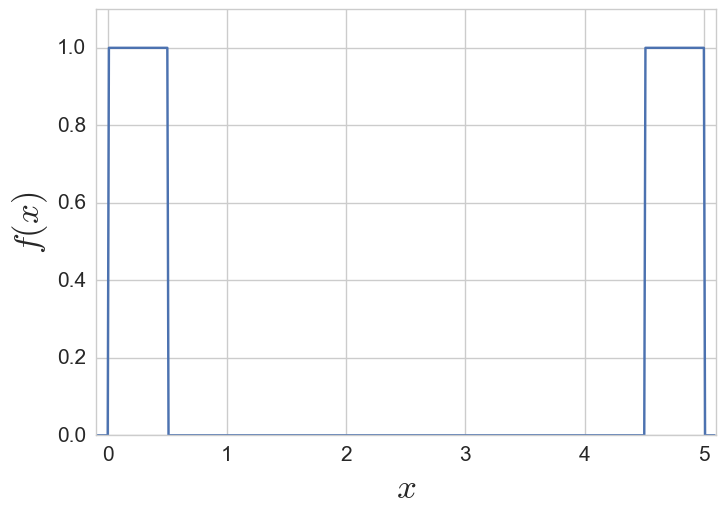
\includegraphics[width=6cm]{problem_distribution.png}
\caption{Pathological distribution for which slice sampling with step out growth $w=1$ will fail.}\label{problem_distribution}
\end{figure}

\end{document}
